% 1. Introducción a la teoría de códigos lineales. 
% Aquí cuanto más quieras leer del libro de Huffman y Pless, mejor. 
% Necesario sólo es el capítulo 1 y el 3 (no todo del 3). 
% Y, aunque no los utilicemos, puedes leerte el capítulo de códigos cíclicos. 
% Es importante centrarse en lo que es la distancia, y que es un problema NP-completo (archivo VARDY.pdf)) ya que es lo que le da seguridad a los criptosistemas.

\chapter{Introducción a la teoría de códigos lineales}

% TODO: reescribir introducción

\textcolor{red}{Hay que reescribir este párrafo}

El inicio de la teoría de códigos surgió a partir de la publicación de Claude Shannon sobre ``Una teoría matemática sobre la comunicación"\ en 1948 \cite{Shannon_1948}. En este artículo, Shannon explica que es posible transmitir mensajes fiables en un canal de comunicación que puede corromper la información enviada a través de él siempre y cuando no se supere la capacidad de dicho canal.

Con la teoría de códigos, podemos codificar datos antes de transmitirlos de tal forma que los datos alterados puedan ser decodificados al grado de precisión especificado. Así, el principal problema es determinar el mensaje que fue enviado a partir del recibido. El Teorema de Shannon nos garantiza que el mensaje recibido coincidirá con el que fue enviado un cierto porcentaje de las veces. Esto hace que el objetivo de la teoría de códigos sea crear códigos que cumplan las condiciones de este teorema.

En esta sección introduciremos los conceptos y resultados fundamentales sobre la teoría de códigos lineales. El desarrollo de este capítulo se ha basado en \cite{Huffman_Pless_2010}, \cite{Vardy_1997}, \cite{Wassermann_2006} y \cite{Podesta_2006}.

\section{Introducción}

Supongamos que queremos enviar un mensaje, por lo que habrá un emisor y un receptor que se comunican en una dirección. Este mensaje es enviado por un \emph{canal de comunicación}, cuyas características dependen de la naturaleza del mensaje a ser enviado. En general, hay que hacer una \emph{traducción} entre el mensaje original (o \emph{palabra fuente}) $x$ y el tipo de mensaje $c$ que el canal está capacitado para enviar (\emph{palabras código}). Este proceso se llama \emph{codificación}. Una vez codificado el mensaje, lo enviamos a través del canal, y nuestro intermediario (el receptor) recibe un mensaje codificado (\emph{palabra recibida}) posiblemente erróneo, ya que en todo proceso de comunicación hay ruido e interferencias. Una vez recibido, empieza el proceso llamado \emph{corrección de errores}, que consiste en recuperar el mensaje original corrigiendo los errores que se hubieran producido. El mensaje recibido $c'$ es traducido nuevamente a términos originales $x'$, es decir, es \emph{decodificado}. La siguiente figura representa un esquema de este proceso.

\begin{figure}[H]
	\center
	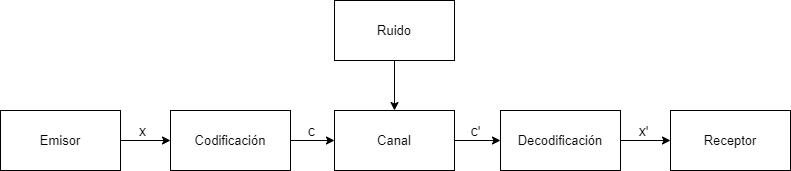
\includegraphics[scale=0.5]{figures/Diagrama_comunicacion.png}
	\caption{Esquema del modelo de comunicación}
\end{figure}

Las flechas indican que la comunicación es en un solo sentido.

En general, $x' \neq x$ y es deseable que este error sea detectado (lo cual permite pedir una retransmisión del mensaje) y en lo posible corregido.

La \emph{Teoría de Códigos Autocorrectores} se ocupa del segundo y cuarto pasos del esquema anterior, es decir, de la codificación y decodificación de mensajes, junto con el problema de detectar y corregir errores. A veces no es posible pedir retransmisión de mensajes y es por eso que los códigos autocorrectores son tan útiles y necesarios.

La calidad de un código con mensajes de longitud $k$ y palabras código de longitud $n$ vendrá dada por las siguientes características.

\begin{itemize}
    \item El cociente $\frac{k}{n}$, el \emph{ratio de información} del código, que mide el esfuerzo necesario para transmitir un mensaje codificado.
    \item La \emph{distancia mínima relativa} $\frac{d}{n}$ que es aproximadamente el doble de la proporción de errores que se pueden corregir en cada mensaje codificado.
    \item La \emph{complejidad} de los procedimientos de codificar y decodificar.
\end{itemize}

De esta forma, uno de los objetivos centrales de la teoría de códigos autocorrectores es construir códigos que sean de calidad. Esto es, códigos que permitan codificar muchos mensajes, que se puedan trasmitir rápida y eficientemente, que detecten y corrijan simultáneamente la mayor cantidad de errores posibles y que haya algoritmos de decodificación fáciles y efectivos. Por lo que habrá que encontrar un balance entre estas distintas metas, pues suelen ser contradictorias entre sí.

\section{Códigos lineales}

Consideramos $\mathbb{F}_q^n$, que denota al espacio vectorial de las n-tuplas sobre el cuerpo finito $\mathbb{F}_q$. Generalmente los vectores $(a_1, ..., a_n)$ de $\mathbb{F}_q^n$ se denotarán por $a_1 \cdots a_n$.

\begin{definition}
    Un $(n, M)$ \emph{código} $\mathcal{C}$ sobre $\mathbb{F}_q$ es un subconjunto de 
    $\mathbb{F}_q^n$ de tamaño $M$. A los elementos de $\mathcal{C}$ los llamaremos \emph{palabras código}.
\end{definition}

\begin{exampleth}
    $ $
    \begin{itemize}
        \item Un código sobre $\mathbb{F}_2$ se llama \emph{código binario} y un ejemplo es $\mathcal{C} = \{00, 01, 10, 11\}$.
        \item Un código sobre $\mathbb{F}_3$ se llama \emph{código ternario} y un ejemplo es $\mathcal{C} = \{21, 02, 10, 20\}$.
    \end{itemize}
\end{exampleth}

Con el fin de aportar más utilidad a los códigos, imponemos linealidad. Así, si $\mathcal{C}$ un subespacio k-dimensional de $\mathbb{F}_q^n$, entonces decimos que $\mathcal{C}$ es un $\left[ n, k \right]$ \emph{código lineal} sobre $\mathbb{F}_q$. De esta forma, los códigos lineales tendrán $q^k$ palabras código. Estos se pueden presentar con una matriz generadora o con una matriz de paridad.

\begin{definition}
    Una \emph{matriz generadora} para un $\left[ n,k \right]$ código $\mathcal{C}$ es una matriz $k \times n$ donde sus filas forman una base de $\mathcal{C}$.
\end{definition}

\begin{definition}
    Para cada conjunto de $k$ columnas independientes de una matriz generadora $G$, se dice que el conjunto de coordenadas correspondiente conforman un \emph{conjunto de información} de $\mathcal{C}$. Las $r = n-k$ restantes coordenadas se denominan \emph{conjunto de redundancia} y el número $r$ es la \emph{redundancia} de $\mathcal{C}$.
\end{definition}

En general, la matriz generadora no es única. Sin embargo, si las $k$ primeras coordenadas conforman un conjunto de información, entonces el código tiene una única matriz generadora de la forma $( I_k | A)$, donde $I_k$ denota a la matriz identidad $k \times k$. Esta matriz se dice que está en \emph{forma estándar}.

Como un código lineal es un subespacio de un espacio vectorial, es el núcleo de alguna transformación lineal.

\begin{definition}
    Una \emph{matriz de paridad} $H$ de dimensión $(n-k) \times n$ de un $\left[ n,k \right]$ código $\mathcal{C}$ se define como

    $$C = \left\lbrace \mathbf{x} \in \mathbb{F} _q^n : H\mathbf{x}^T = 0 \right\rbrace .$$
\end{definition}

Al igual que con la matriz generadora, la matriz de paridad no es única. Con el siguiente resultado podremos obtener una matriz de paridad cuando $\mathcal{C}$ tiene una matriz generadora en forma estándar.

\begin{theorem}
    \label{th:generadora-paridad}
    Si $G = \left( I_k | A \right)$ es una matriz generadora para el $\left[ n,k \right]$ código $\mathcal{C}$ en forma estándar, entonces $H = \left( -A^T | I_{n-k} \right)$ es una matriz de paridad de $\mathcal{C}$.
\end{theorem}

\begin{proof}
    Como $HG^T = -A^T + A^T = 0$, se tiene que $\mathcal{C}$ está contenido en el núcleo de la transformación lineal $x \mapsto Hx^T$. Esta transformación lineal tiene un núcleo de dimensión $k$, pues $H$ tiene rango $n-k$, que coincide con la dimensión de $\mathcal{C}$.
\end{proof}

\begin{exampleth}
    \label{ex:generadora-paridad}
    Sea la matriz $G = \left( I_4 | A \right)$, donde 
    
    \[
        G = \left( 
        \begin{array}{cccc|ccc}  
            1 & 0 & 0 & 0 & 0 & 1 & 1 \\
            0 & 1 & 0 & 0 & 1 & 0 & 1 \\
            0 & 0 & 1 & 0 & 1 & 1 & 0 \\
            0 & 0 & 0 & 1 & 1 & 1 & 1
        \end{array} 
        \right)
    \]

    es una matriz generadora en forma estándar para un $[7, 4]$ código binario que denotaremos por $\mathcal{H}_3$. Por el Teorema \ref{th:generadora-paridad}, una matriz de paridad de $\mathcal{H}_3$ es

    \[ 
        H = 
        \left( 
        \begin{array}{c|c}  
            -A^T & I_{7-4}
        \end{array} 
        \right)
        = 
        \left( 
        \begin{array}{c|c}  
            -A^T & I_{3}
        \end{array} 
        \right)
        =
        \left( 
        \begin{array}{cccc|ccc}  
            0 & 1 & 1 & 1 & 1 & 0 & 0 \\
            1 & 0 & 1 & 1 & 0 & 1 & 0 \\
            1 & 1 & 0 & 1 & 0 & 0 & 1 \\
        \end{array} 
        \right)
    \]
\end{exampleth}

\section{Código dual}

Sabemos que $\mathcal{C}$ es un subespacio de un espacio vectorial, por lo que podemos calcular un subespacio ortogonal a dicho subespacio y así obtener lo que se denomina \emph{espacio dual u ortogonal} de $\mathcal{C}$, denotado por $\mathcal{C} ^{\perp}$. Se define este concepto con la operación del producto escalar como sigue.

\begin{definition}
    El \emph{espacio dual} de $\mathcal{C}$ viene dado por 
    
    $$\mathcal{C} ^{\perp} = \left\{ \mathbf{x} \in \mathbb{F}_q^n \; : \; \mathbf{x} \cdot \mathbf{c} = 0 \quad \forall \mathbf{c} \in \mathcal{C} \right\}$$
\end{definition}

Se observa que $\mathcal{C} ^{\perp}$ es un $[n,n-k]$ código.

El siguiente resultado nos muestra cómo obtener las matrices generadora y de paridad de $\mathcal{C} ^{\perp}$ a partir de las de $\mathcal{C}$.

\begin{proposition}
    Si tenemos una matriz generadora $G$ y una matriz de paridad $H$ de un código $\mathcal{C}$, entonces $H$ y $G$ son matrices generadoras y de paridad, respectivamente, de $\mathcal{C} ^{\perp}$.
\end{proposition}

Diremos que un código $\mathcal{C}$ es \emph{auto-ortogonal} si $\mathcal{C} \subseteq \mathcal{C} ^{\perp}$ y \emph{auto-dual} cuando $\mathcal{C} = \mathcal{C} ^{\perp}$.

\begin{exampleth}
    Una matriz generadora para el $[7, 4]$ código de Hamming $\mathcal{H}_3$ se presenta en el Ejemplo \ref{ex:generadora-paridad}. Sea $\mathcal{H'}_3$ el código de longitud 8 y dimensión 4 obtenido de $\mathcal{H}_3$ añadiendo una coordenada de verificación de paridad general a cada vector de G y por lo tanto a cada palabra código de $\mathcal{H}_3$. Entonces 

    \[
        G' = \left( 
        \begin{array}{cccc|cccc}  
            1 & 0 & 0 & 0 & 0 & 1 & 1 & 1 \\
            0 & 1 & 0 & 0 & 1 & 0 & 1 & 1\\
            0 & 0 & 1 & 0 & 1 & 1 & 0 & 1\\
            0 & 0 & 0 & 1 & 1 & 1 & 1 & 0
        \end{array} 
        \right)
    \]

    es una matriz generadora para $\mathcal{H'}_3$. Además, veamos que $\mathcal{H'}_3$ es un código auto-dual.

    Tenemos que $G' = (I_4 | A')$, donde

    \[
        A' = \left( 
        \begin{array}{cccc}  
            0 & 1 & 1 & 1 \\
            1 & 0 & 1 & 1\\
            1 & 1 & 0 & 1\\
            1 & 1 & 1 & 0
        \end{array} 
        \right) .
    \]

    Como $A' (A')^T = I_4$, entonces $\mathcal{H'}_3$ es auto-dual.
\end{exampleth}

\section{Pesos y distancias}

Es importante saber lo que difieren las palabras código. En este apartado estudiaremos esta idea y cómo puede influir a la teoría de códigos.

\begin{definition}
    La \emph{distancia de Hamming} $\operatorname{d}(\mathbf{x},\mathbf{y})$ entre dos vectores $\mathbf{x}$, $\mathbf{y} \in \mathbb{F}_q^n$ se define como el número de coordenadas en las que $\mathbf{x}$ e $\mathbf{y}$ difieren.
\end{definition}

\begin{exampleth}
    Sean $\mathbf{x} = 012$, $\mathbf{y} = 210$ $\mathbf{x}, \mathbf{y} \in \mathbb{F}_3^4$. Entonces la distancia de Hamming entre los dos vectores es $d(\mathbf{x}, \mathbf{y}) = 2$.
\end{exampleth}

\begin{theorem}
    La función distancia $\operatorname{d}(\mathbf{x},\mathbf{y})$ satisface las siguientes propiedades.

    \begin{enumerate}
        \item No negatividad: $\operatorname{d}(\mathbf{x},\mathbf{y}) \geq 0 \quad \forall \mathbf{x},\mathbf{y} \in \mathbb{F}_q^n$.
        \item $\operatorname{d}(\mathbf{x},\mathbf{y}) = 0 \; \Leftrightarrow \; \mathbf{x} = \mathbf{y}$.
        \item Simetría: $\operatorname{d}(\mathbf{x},\mathbf{y}) = \operatorname{d}(\mathbf{y},\mathbf{x}) \quad \forall \mathbf{x},\mathbf{y} \in \mathbb{F}_q^n$.
        \item Desigualdad triangular: $\operatorname{d}(\mathbf{x},\mathbf{z}) \leq \operatorname{d}(\mathbf{x},\mathbf{y}) + \operatorname{d}(\mathbf{y},\mathbf{z}) \quad \forall \mathbf{x},\mathbf{y},\mathbf{z} \in \mathbb{F}_q^n$
    \end{enumerate}
\end{theorem}

\begin{proof}
    Las tres primeras afirmaciones se obtienen directamente a partir de la definición.
    La cuarta propiedad se obtiene a partir de la no negatividad. Esto es, sean $x,y,z \in \mathbb{F}_q^n$ distingamos dos casos. Si $x \neq z$
    tenemos que $y \neq x$ o $y \neq z$, entonces por la no negatividad se cumple la afirmación.
    En el caso en el que $x = z$, tendríamos que $d(x,z) = 0$ y también se da la 
    afirmación.
\end{proof}

Diremos que la \emph{distancia mínima} de un código $\mathcal{C}$ es la distancia más pequeña entre las distintas palabras código. Esta medida es fundamental a la hora de determinar la capacidad de corregir errores de $\mathcal{C}$.

\begin{exampleth}
    Sea $\mathcal{C} = {010101, 212121, 111000}$ un código ternario. Entonces

    $$d(010101, 212121) = 3, \qquad d(010101, 111000) = 4, \qquad d(212121, 111000) = 5.$$

    Por lo que la distancia mínima del código $\mathcal{C}$ es $d(\mathcal{C}) = 3$.
\end{exampleth}

\begin{theorem}[Decodificación de máxima verosimilitud]
    \label{th:decodificacion_maxima_verosimilitud}
    Es posible corregir hasta

    $$t := \left\lfloor \frac{d(\mathcal{C}) - 1}{2} \right\rfloor$$

    errores, donde $d(\mathcal{C})$ denota la distancia mínima del código $\mathcal{C}$.
\end{theorem}

\begin{proof}
    Usando la decodificación de máxima verosimilitud, un vector $y \in \mathbb{F}^n$ es decodificado en una palabra código $c  \in \mathcal{C}$, que es cercana a $y$ con respecto a la distancia de Hamming. Formalmente, $y$ es decodificado en una palabra código $c \in \mathcal{C}$ tal que $d(c,y) \leq d(c',y)$, $\forall c' \in \mathcal{C}$. Si hay varios $c \in \mathcal{C}$ con esta propiedad, se elige uno arbitrariamente.

    Si la palabra código $c \in \mathcal{C}$ fue enviada y no han ocurrido más de $t$ errores durante la transmisión, el vector recibido es 

    $$y = c + e \in \mathbb{F}^n,$$

    donde $e$ denota al vector error. Esto satisface 

    $$d(c,y) = d(e,0) \leq t,$$

    y por lo tanto $c$ es el único elemento de $\mathcal{C}$ que se encuentra en una bola de radio $t$ alrededor de $y$. Un decodificador de máxima verosimilitud produce este elemento $c$, y así se obtiene el código correcto.
\end{proof}

\begin{definition}
    El \emph{peso Hamming} $\operatorname{wt}(\mathbf{x})$ de un vector $\mathbf{x} \in \mathbb{F}_q^n$ se define como el número de coordenadas no nulas en $\mathbf{x}$.
\end{definition}

\begin{exampleth}
    Sea $\mathbf{x} = 2001021 \in \mathbb{F}_3^7$ un vector, entonces su peso Hamming es $wt(\mathbf{x}) = 4$.
\end{exampleth}

El siguiente resultado nos muestra la relación entre la distancia y el peso.

\begin{theorem}
    Si $\mathbf{x}, \mathbf{y} \in \mathbb{F}_q^n$, entonces $\operatorname{d}(\mathbf{x},\mathbf{y}) = \operatorname{wt}(\mathbf{x}-\mathbf{y})$. Si $\mathcal{C}$ es un código lineal, entonces la distancia mínima $d$ coincide con el peso mínimo de las palabras código no nulas de $\mathcal{C}$.
\end{theorem}

\begin{proof}
    Sean $x,y \in \mathbb{F}_q^n$, por la definición de distancia de Hamming tenemos que $d(x,y) = wt(x-y)$. Se supone ahora que $C$ es un código lineal, luego para todo $x,y \in \mathcal{C}$, $x-y \in \mathcal{C}$, luego para cualquier par de elementos $x,y \in \mathcal{C}$, existe $z \in \mathcal{C}$ tal que $d(x,y) = wt(z) \geq wt(\mathcal{C})$, donde $wt(\mathcal{C})$ es el peso mínimo de $\mathcal{C}$. Por tanto, $d \geq wt(\mathcal{C})$. Por otro lado, para todo $x \in \mathcal{C}$, se tiene que $wt(x) = d(x,0)$. Como $\mathcal{C}$ es lineal, $0 \in \mathcal{C}$, luego $d(x,0) \geq d$. Entonces, $wt(\mathcal{C}) \geq d$. Se concluye que $wt(\mathcal{C}) = d$, como se quería.
\end{proof}

Como consecuencia de este teorema, para códigos lineales, la distancia mínima también se denomina \emph{peso mínimo} de un código. Si se conoce el peso mínimo $d$ de un $[n,k]$ código, se denota por un $[n,k,d]$ código.

Se ha demostrado que el problema de calcular la distancia mínima de un código lineal binario es NP-difícil, y el problema de decisión correspondiente es NP-completo. Esto es, formalmente, dada una matriz binaria $H$ de dimensión $m \times n$ y un número entero $w > 0$, saber si existe un vector no nulo $x \in \mathbb{F}_2^n$ de peso menor que $w$ tal que $Hw^T = 0$ es un problema NP-completo. 

\begin{proof}
    Para ello, haremos uso de una transformación polinomial del problema de Decodificación de Máxima Verosimilitud al problema de Distancia Mínima.

    El problema de Decodicificación de Máxima Verosimilitud es NP-completo y consiste en dados una matriz binaria $H$ de dimensión $m \times n$, un vector $s \in \mathbb{F}_2^m$ y un número entero $w > 0$. ¿Existe un vector $x \in \mathbb{F}_2^n$ de peso menor o igual que $w$ tal que $Hx^t = s$?

    El problema de Decodificación de Máxima Verosimilitud sigue siendo NP-completo bajo ciertas restricciones, luego reformularemos este problema como la versión de campo finito de Suma de Subconjuntos, un problema NP-completo conocido. Además, calcular la distancia mínima para la clase de códigos lineales sobre un cuerpo de característica 2 es NP-difícil, y el problema de decisión correspondiente Distancia Mínima sobre $GF(2^m)$, abreviado $MD_{2^m}$, es NP-completo. Luego esta prueba se basa en una transformación polinomial de Decodificación de Máxima Verosimilitud a $MD_{2^m}$. Sin embargo, esto no prueba que Distancia Mínima sea NP-completo, ya que el posible conjunto de entradas a Distancia Mínima es un pequeño subconjunto del conjunto de posibles entradas a $MD_{2^m}$. Para ello, se construye una aplicación del código $\mathbb{C\#}$ sobre $GF(2^m)$ a un código binario $\mathbb{C}$, de tal forma que la distancia mínima de $\mathbb{C\#}$ puede determinarse a partir de la distancia mínima de $\mathbb{C}$. Dado que la longitud de $\mathbb{C}$ está acotada por la longitud de un polinomio de $\mathbb{C\#}$, y el mapeo en sí se puede lograr en tiempo polinomial, esto completa la prueba de la NP-completitud de Distancia Mínima.
\end{proof}

Como hemos visto, la distancia mínima es importante en un código lineal. Sin embargo, calcular este parámetro para un código dado puede resultar realmente duro. A continuación presentaremos un algoritmo para el cálculo de la distancia.

\begin{Ualgorithm}[htbp]
    \DontPrintSemicolon
    \KwIn{matriz generadora $G_1 = (I_k | A_1)$ de $\mathcal{C}$}
    \KwOut{distancia mínima $\bar{d}_i$}
    $m \longleftarrow 2$\;
    $k_1 \longleftarrow k$\;
    \While{rank $(A_m) \neq 0$}{
        Aplicar la eliminación Gaussiana y posibles permutaciones de las columnas de la matriz $A_{m-1}$ desde $G_{m-1} = \left( \begin{array}{c|c} A_{m-1}' & \begin{array}{c|c} I_{k_{m-1}} & A_{m-1} \\ \hline  0 & 0 \end{array} \end{array} \right)$ para obtener la matriz generadora $G_{m} = \left( \begin{array}{c|c}  A_{m}' & \begin{array}{c|c}   I_{k_{m}} & A_{m} \\  \hline 0 & 0  \end{array}  \end{array} \right)$\;
    }
    $C_0 \longleftarrow \left\lbrace 0 \right\rbrace$\;
    $i \longleftarrow 0$\;
    \While{$\bar{d}_i > d_i'$}{
        $i \longleftarrow i + 1$\;
        $C_i \longleftarrow C_{i-1} \cup \bigcup_{j=1}^m \left\lbrace v \cdot G_j : v \in \mathbb{F}(q)^k, \; wt(v) = i \right\rbrace$\;
        $\bar{d}_i \longleftarrow min \lbrace wt(c) : c \in C_i, \; c \neq 0 \rbrace$\;
        $d_i' \longleftarrow \sum_{j=1, k-k_j \leq i}^m (i+1)-(k-k_j)$\;
    }
    \caption{Algoritmo de Brouwer-Zimmermann: cálculo de la distancia mínima de un $[n,k]$ código lineal $\mathcal{C}$.}
\end{Ualgorithm}

\begin{definition}
    Sea $A_i$, también denotada por $A_i(\mathcal{C})$, el número de palabras código con peso $i$ en $\mathcal{C}$. Se dice que la lista $A_i$ para $0 \leq i \leq n$ es la distribución del peso o espectro del peso de $\mathcal{C}$.
\end{definition}

\section{Clasificación por isometría}

Como hemos visto, las propiedades de codificación de un código dependen principalmente de las distancias de Hamming entre diferentes palabras codificadas y entre palabras codificadas y no codificadas. Además, puede ser que un código pueda relacionarse con otro por medio de una aplicación que conserve las distancias de Hamming. De esta forma, podemos definir una relación de equivalencia entre dos códigos que preservan la distancia de Hamming.

Tenemos que dos $(n,k)$-códigos $C, C' \subseteq H(n,q)$ son de la misma cualidad si existe un mapeo

$$\iota : H(n,q) \rightarrow H(n,q)$$

con $\iota(C) = C'$ que preserva la distancia de Hamming, es decir, 

$$d(w,w') = d(\iota (w), \iota(w')), \qquad \forall w,w' \in H(n,q).$$

Los mapeos con la propiedad anterior se llaman \emph{isometrías}.

\begin{definition}
    Dos códigos lineales $C, C' \subseteq H(n,q)$ se llaman \emph{isométricos} si existe una isometría de $H(n,q)$ que aplica $C$ sobre $C'$.
\end{definition}

Las permutaciones de las coordenadas son isometrías, que se denominan \emph{isometrías permutacionales}.

\begin{definition}
    Sea $S_n$ el grupo isométrico en el conjunto $X = n = \left\{ 0,..., n-1 \right\}$. Dos códigos lineales $C, C' \subseteq H(n,q)$ son isométricos permutacionalmente si existe una isometría permutacional de $H(n,q)$ que aplica $C$ sobre $C'$. Esto es, hay una permutación $\pi$ en el grupo simétrico $S_n$ tal que 

    $$ C' = \pi (C) = \left\{ \pi(c) : c \in C \right\}, \quad \text{ and } \quad d(c, \tilde{c}) = d(\pi(c), \pi(\tilde{c})), \qquad \forall c,\tilde{c} \in C,$$ 

    donde
    
    $$\pi(c) = \pi(c_0,...,c_{n-1}) := \left( c_{\pi ^{-1} (0)}, ..., c_{\pi ^{-1} (n-1)} \right)$$
\end{definition}
